\chapter{Experimental results \status{in progress}}
\label{chap:results}

In this chapter we quantitatively and qualitatively analyse the performance of the automatic cell detector and tracker. Although some evaluation of the performance of the detection method is performed by the original authors in \cite{arteta12} it is useful to see how the method performs on the studied datasets in order to understand how much of the tracking accuracy is lost due to cells missed by detection module. First, in \cref{sec:results_detector} we evaluate the performance and computation time of the cell detector and in \cref{sec:results_tracker} those of the cell tracker. Finally, in \cref{sec:results_limitations}, we explore the limitations of the methods and in \cref{sec:results_summary} summarize the results.

\todo[inline]{See the cell population tracking and linear construction with spationtemporal ocntet by Kang et al for a good results section}

	\section{Cell detector \status{in progress}}
		\label{sec:results_detector}
		
		In this section we evaluated the performance of the automatic cell detection module. First, we introduce the performance metrics used to evaluate the accuracy of the cell detector. Then we present detection accuracy results. To evaluate the accuracy and generalizability of the detection module we perform two sets of experiments. First, we train the cell detector on a number of frames from each individual dataset, and measure the accuracy on the same dataset. Second, we train the detector on combinations of datasets in order to judge the performance degradation due to the learning on the wider types of cells. Because of the varying size of the cells in the datasets, and the varying brightness of the cells, we expect that such a trained detector will detect a larger number of cells than are actually present, sometimes mistakenly detecting small artefacts in the background as cells. Finally, we compute the average detection time per frame for each dataset.
		
		The aim of this research was to develop an automatic cell detection and tracking pipeline that would require as little manual work as possible. This implies that a balance between accuracy and amount of manual work had to be established. There is also an direct relationship between accuracy and computation time. In order to reduce the amount of manual work we decided that the cell detection module should perform well on all the tested datasets without any manual adjustment of parameters. This consequences of this decision are twofold:
		
		\begin{enumerate}
			\item The features computed on the candidate cell regions are the same for all datasets and have been presented in \cref{sec:detector_feature}. Although some datasets could be analysed faster or more accurately with a different subset of features, using the same features for all dataset eliminates the complicated feature selection process for the user and makes the system generalizable to a large number of different cell types.
			
			\item The parameters of the MSER detector should be adequately set to perform well on all datasets. This means that the MSER detector should be able to detect cells of varying size and contrast in the different datasets. The consequence of this limitation for datasets with bigger cells and some background noise is that a potentially much larger number of candidate regions will be detected than necessary. Since each candidate region has to be evaluated this results in an increased computation time.
		\end{enumerate}
		
		We were able to identify features that compute in an acceptable time for all these datasets (see \cref{sec:detector_feature}). However, it should be noted that in the case of testing the detector on very large datasets with thousands of frames, some adjustments of the parameters could result in a significant reduction in computation time and increased accuracy.
		
		\subsection{Performance metrics \statusnew}
			precision, recall, time per image (not multicore)
		
		Figure \ref{fig:cell_tracks_detection} displays a temporal view of the detected cells. The vertical axis represents the frame of the sequence. The figure clearly shows that ``cell tracks'' are clearly discernible, even if the number of outliers is significant. For the tracking module it is better to have a higher recall than precision, as outliers can be much more easily discarded than segmented tracks linked.
		\begin{figure}
			  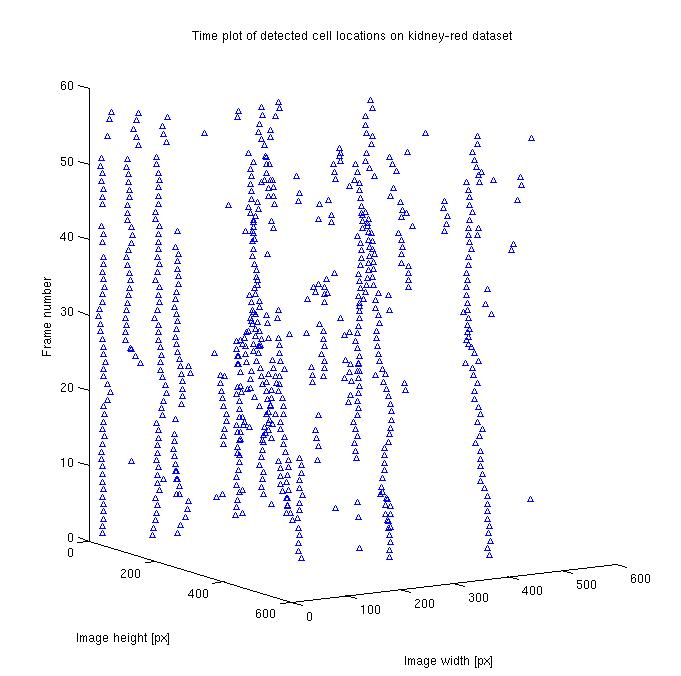
\includegraphics[width=\textwidth]{images/cell_tracks}
			\caption{Cells detected over 60 consecutive frames are visualized as a time series. The vertical axis corresponds to the frames. Even in this raw detection data, it is possible to see the tracks of some of these cells.}
		    \label{fig:cell_tracks_detection}
		\end{figure}
		

		
		\subsection{Detection accuracy \statusnew}
			
			- trained on single dataset
			
			- trained on combined dataset
			
		\subsection{Computations time \statusnew}
			explain hardware, software 
			\todo[inline]{Measure the speed of detection in images of different sizes, and different number of cells}
	\section{Cell tracker \statusnew}
		\label{sec:results_tracker}
		\todo[inline]{Define the different measures of accuracy}
		\subsection{Performance metrics \statusnew}
		
		great Metrics: Research Article, Evaluating Multiple Object Tracking Performance: The CLEAR MOT Metrics
		
		- Explain how the testing data was generation. from annotation to mapped deteciton to genreated tracklets
		\subsection{Computation time \statusnew}
		\todo[inline]{Meause the speed of generating tracks, as a measure of per 1, 100, 1000 frames, depending on the number of tracks}
		\subsection{Tracking accuracy \statusnew}
			
		
			- trained on single dataset
			
			- for each dataset explain how the parameters were setup
						
			- trained on combined dataset
	\section{Limitations and areas of improvement \statusnew}
		\label{sec:results_limitations}
		Answer: what, why, how to improve in future
				
		- display examples where the tracker did not perform well, and anlyse why. Suggest possible improvement.
		- detection training: only first few frames of datasets, not random -- expect to detect later frames worse
		- testing on only long datasets: no data on short datasets. diffucult to train (what to link?), difficult to annotate
		- speed of detector. Reduce number of hypothesis		

	\section{Summary \statusnew}
		\label{sec:results_summary}
		Brief review of accuracy... whether it is comparable to other methods in literuature review
		Whether is could be improved in the future... how much